\chapter{Complex morphology of the northern jet: An effect of jet precession}\label{chapter7}


Hydra A, located at the centre of the galaxy cluster Abell 780, shows a spectacular S-shaped morphology within the central 20~kpc. The symmetrical S-structure is also visible in the extended low frequency images at 74 and 330~MHz \citep{lane04}. The radio source is extended by approximately 340~kpc in the north and by 190~kpc in the south. Modelling the entire source is computationally impractical and I have adopted the approach of modelling the innermost structures (inner 10~kpc of the northern jet) first in order to constrain jet parameters (see chapter~\ref{chapter5}), then utilising these parameters model the intermediate scale structure (inner 20~kpc of the northern jet). 

I have studied the kinetic power of the Hydra A jets and two key features of the inner 10~kpc of the northern jet: i) the oscillatory jet boundary and ii) two bright knots at approximately 3.7~kpc and 7.0~kpc (see chapters~\ref{chapter3} and \ref{chapter5}). Since the jet is mildly bent within 10~kpc, I have used two dimensional axisymmetric simulations and have modelled the inner two bright knots as biconical reconfinement shocks. By fitting the knot location and the radius profile of the modelled and observed jet I have estimated the jet velocity at 0.5~kpc to be approximately 0.8c, the jet over pressure ratio  with respect to the ICM approximately 5, the jet density parameter approximately 13. 

In this chapter I address the following additional key features of the inner 20~kpc of the northern Hydra A jet: i) the curved jet morphology, ii) two additional bright knots beyond 10 kpc and iii) the turbulent transition of the jet to a dissipative plume. In Fig.~\ref{f:obs} I show the radio structure of the northern jet and indicate these features. This figure is produced using the 4.635~GHz VLA data (G. Taylor, priv. comm.).  The detailed description of these data is available in \citet{taylor90}. In order to model the curved jet morphology I use a three dimensional hydrodynamical model of a precessing jet based on the jet and interstellar medium (ISM) parameters obtained in chapter~\ref{chapter5}. 

%%%%%%%%%%%%%%%%%%%%%%%%%%%%%%%%%%%%%%%%%%%%%%%%%%%%%%%%%%%%%%%%%%%%%%%%
%
%												Details of the model
%
%%%%%%%%%%%%%%%%%%%%%%%%%%%%%%%%%%%%%%%%%%%%%%%%%%%%%%%%%%%%%%%%%%%%%%%%
\section{Details of the model}\label{s:model}
\begin{figure*}
\centering
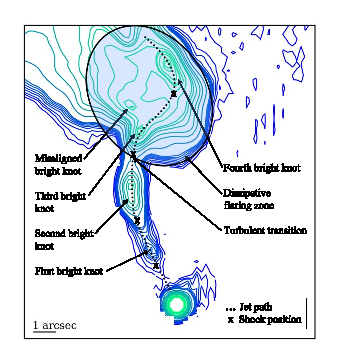
\includegraphics[width=10cm]{fig1.eps}
\caption{Radio intensity map of the central 20~kpc of the Hydra A northern jet at 4.635 GHz. Contour levels are at 1.5, 2.7, 3.7, 5.1, 6.3, 7.5, 8.8, 10, 21, 37, 51, 72, 90, 103, 150, 180, 200, 205, 220, 240 and 249 mJy arcsec$^{-2}$. Four bright knots are marked with black arrows. The locations of the biconical reconfinement shocks which I interpret as the cause of the bright knots \citep{nawaz14a} are marked with $\times$. An imaginary jet path is traced by a dotted line following the ridge line and joining the four knots. Near the third knot there is a bright knot, marked as 'misaligned knot', which is not aligned with the jet trajectory. The turbulent transition of the jet starts at the location marked by an arrow. The elliptical shaded area outline a dissipative zone.}
\label{f:obs}
\end{figure*}

The motivation for this study is to understand the dynamical interaction of the inner Hydra A northern jet with the interstellar medium and cluster environment and to understand the reason for the source morphology. Therefore, I mainly focus on the features of the inner 20~kpc including i) the curved jet ii) the four bright knots at approximately 3.7~kpc, 7.0~kpc, 11.0~kpc and 16.0~kpc from the core (deprojected) iii) the turbulent transition of the jet to a plume at approximately 10~kpc from the core, and iv) the bright radio emission region at approximately 10 to 20~kpc from the core. 

In chapter~\ref{chapter5} using axisymmetric straight jet simulations I modelled the first two bright knots of the northern jet as biconical reconfinement shocks. Here I develop this model by introducing precession of the jet and this necessitates three dimensional simulations.  According to my model, the jet is initially ballistic and conically expands in the first 0.5~kpc. It then starts to interact with the ISM and is collimated by the ambient pressure. A series of bright knots are produced along the jet path at the locations of the biconical reconfinemnet shocks. 

The initially supersonic jet is decelerated significantly by the first two reconfinement shocks and the jet starts to form a turbulent plume at approximately 11~kpc from the core. The jet strongly interacts with the ISM and produces further reconfinement shocks at approximately 11~kpc and 16~kpc. Some jet plasma is deflected by the dense cocoon wall near the fourth knot and a highly turbulent zone is established in the region approximately 11-20~kpc from the core. 

Note that in the northern Hydra A jet there is a bright knot (marked by 'mis-aligned knot') that is not aligned with the jet path (the black dotted line in Fig.~\ref{f:obs} inferred by following the ridge line and connecting the four bright knots). Prior to conducting the simulations there was no indication as to how this misaligned knot actually formed. 

My modelling strategy is as follows: I conduct a small parameter space study with jet parameters derived from the best fit axisymmetric model of Paper I, a range of precession periods and two values of the precession angle.  I then construct synthetic surface brightness images of the models and compare the source morphology obtained from my models with the observations. Matching the key features, namely, the curvature of the jet, the locations of the bright knots and the turbulent transition of the jet to a plume, I select a best model. 

The input jet parameters, the jet kinetic power $P_{\rm jet} = 1\times 10^{45}$~erg s$^{-1}$, the jet over-pressure ratio $p_{\rm jet}/p_{\rm a} = 5$, the jet velocity $\beta = 0.8$, and the jet density parameter $\chi = 12.75$ are chosen from the best fit axisymmetric model presented in Paper I. I explore a range of values for the precession period $P = 1, 5, 10, 15, 20, 25$~Myr and the precession angle $\theta = 15^{\circ} \rm \ and \ 20^{\circ}$. The grid of models is presented in Table~\ref{t:mod}. Since the radiative cooling timescale of the jet plasma and ambient medium are large compared to the simulation time, I do not include cooling in my models. 

%%%%%%%%%%%%%%%%%%%%%%%%%%%%%%%%%%%%%%%%%%%%%%%%%%%%%
%
%						Numerical Setup
%
%%%%%%%%%%%%%%%%%%%%%%%%%%%%%%%%%%%%%%%%%%%%%%%%%%%%%
\begin{table*}
\centering
\caption{Grid of precessing jet-ICM interaction model. }
%\begin{threeparttable}
\begin{tabular}{*{7}{c}}
\hline \hline
%GVB
% Models &   $P$ & $\theta$  & Computation domain  \\
Model &   Period & Precession   \\
      & (Myr)  & angle (degrees) \\ 
 \\ \hline
   A & 1.0 & 20 \\
   B & 1.0 & 15  \\
   C & 5.0  & 20  \\
   D & 10.0 & 20 \\
   E & 15.0 & 20 \\
   F & 20.0 & 20 \\
   G & 25.0 & 20 \\
\hline
\end{tabular}
\label{t:mod}
%\end{threeparttable}
\end{table*}

%%%%%%%%%%%%%%%%%%%%%%%%%%%%%
%
%			Synthetic surface brightness
%
%%%%%%%%%%%%%%%%%%%%%%%%%%%%%
\subsection{Synthetic surface brightness}
\begin{figure*}
\centering
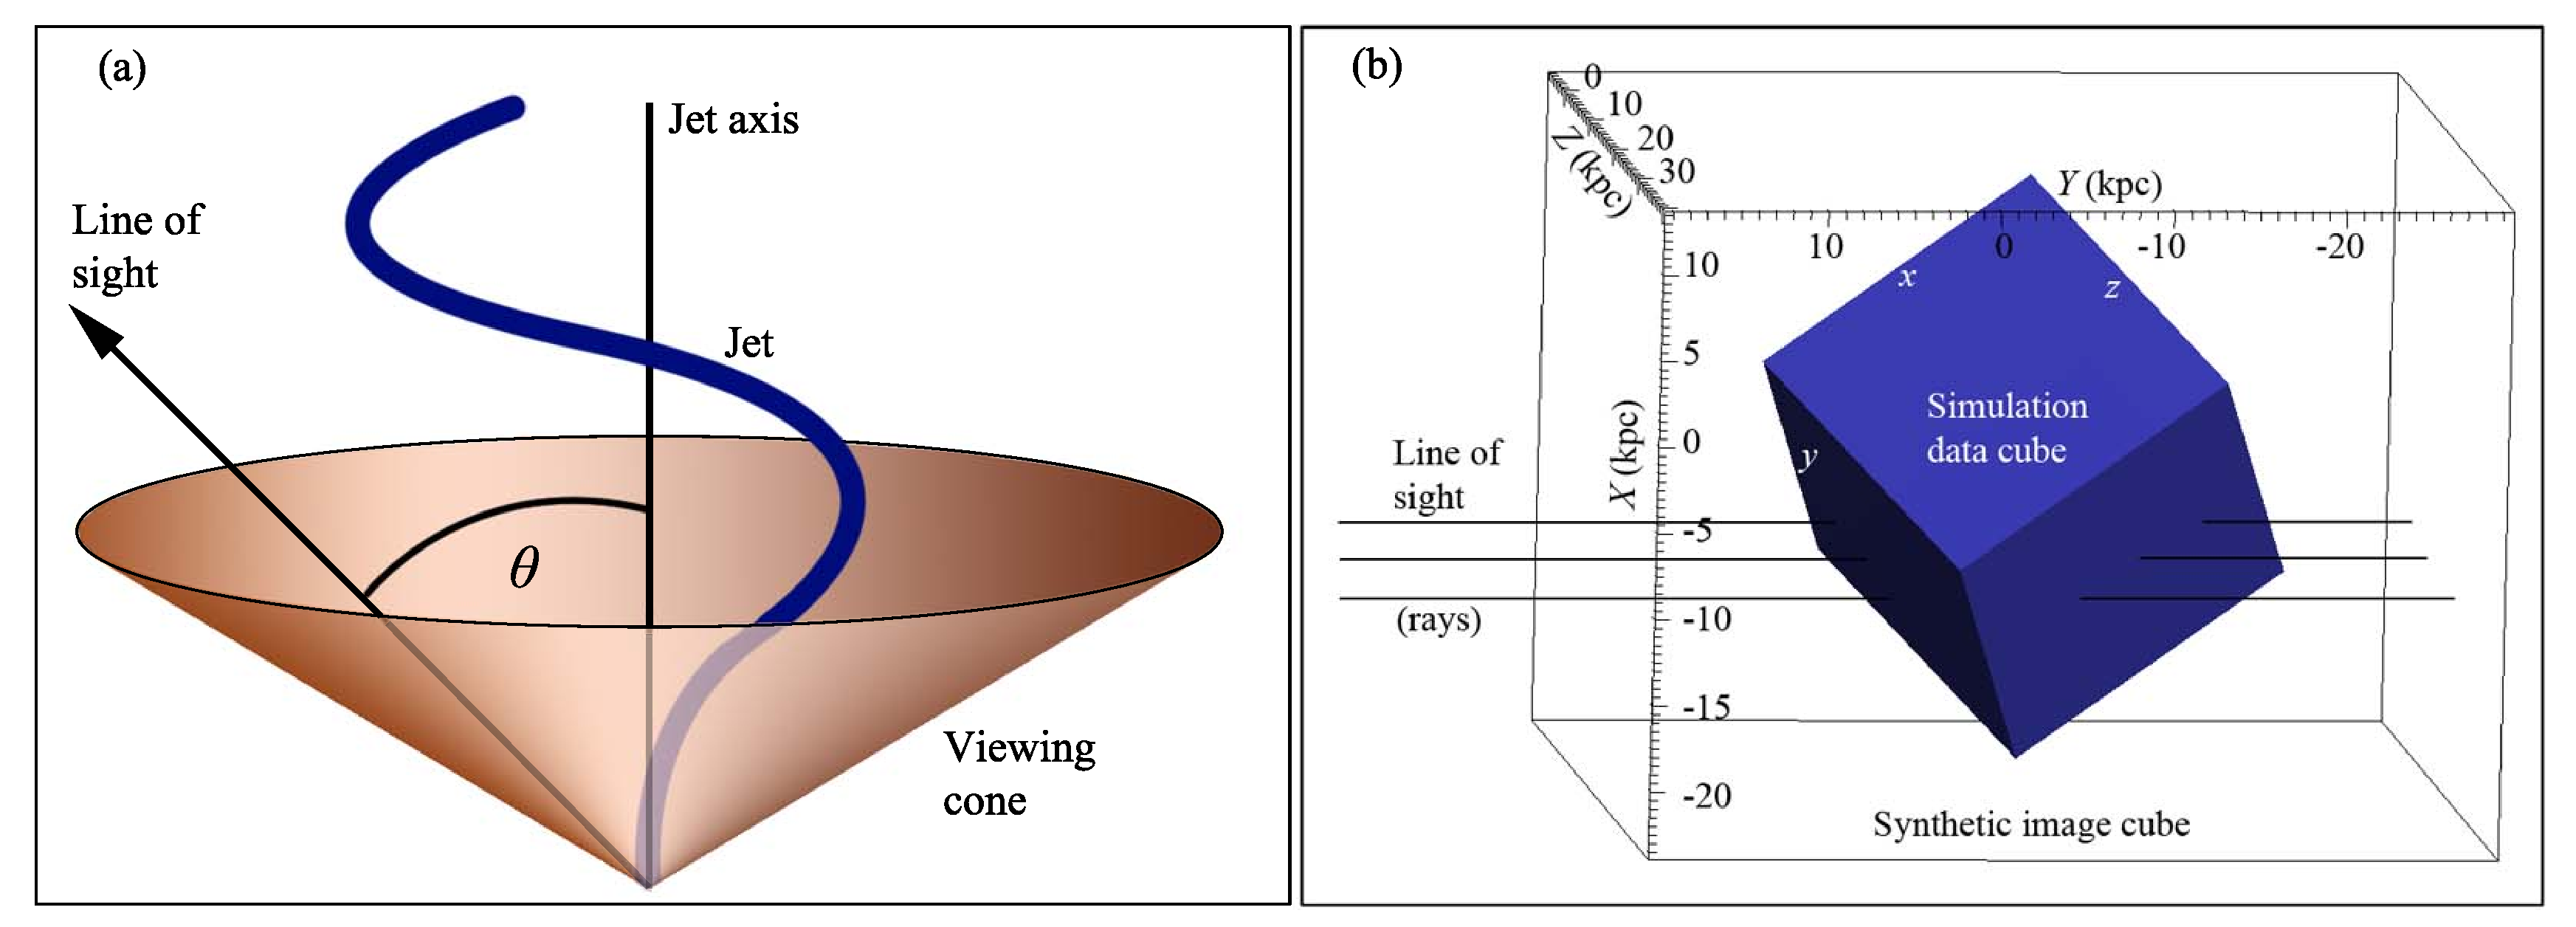
\includegraphics[width=\textwidth]{fig3.eps}
\caption{Dependencies of the jet morphology on the line of sight and the viewing direction. (a) A cartoon of a spiral jet, an arbitrary line of sight and a viewing cone with cone axis aligned with the jet axis and cone angle equal to the line of sight angle are shown. Any line of sight lying on the viewing cone has the same inclination $\theta$ with the jet axis. The observed source morphology depends on both the line of sight inclination $\theta$ and the viewing direction. (b) The image cube, the data cube and the line of sight (marked by rays) are shown. The data cube is rotated with respect to the image cube to obtain any line of sight and a viewing direction.}
\label{f:con}
\end{figure*}

In order to compare the morphologies derived from the models with the radio observations I produce synthetic surface brightness images for each model. Following \citet{sutherland07}, I use a synchrotron rest-frame emissivity $j_\nu \propto p^{(3+\alpha)/2}$ where  $\alpha$ is the spectral index.  In this expression, the magnetic pressure is assumed to be proportional to the non-thermal particle pressure. The northern Hydra A jet is approaching towards the observer and hence the emissivity $j_\nu$ is modified by the Doppler factor $\delta = 1/\Gamma(1 - \beta \cos\theta]$, where $\Gamma$ is the bulk Lorentz factor and $\theta$ is the angle between the jet axis and the line of sight. In addition, to isolate the jet plasma from the ambient medium I use a tracer $\lambda$, which is the mass concentration of plasma at each cell. I initialise the jet plasma with a value $\lambda = 1$. Hence the emissivity $j_\nu$ becomes (in arbitrary units) 
\begin{equation}
j_\nu = \lambda \delta^{2+\alpha}p^{(3+\alpha)/2}
\end{equation}
Integrating the synchrotron emissivity along rays, parallel to the line of sight, $I_\nu = \int j_\nu ds$, I obtain images of the synthetic surface brightness (in arbitrary units) of the modelled jets. 

I note that the source morphology depends on both the angle between the jet axis and the line of sight and the viewing direction in azimuth. For instance, Fig.~\ref{f:con} shows an arbitrary spiral jet structure about the jet axis and an arbitrary line of sight (making an angle $\theta$ with the jet axis). In this figure a viewing cone is also shown. The axis of the viewing cone lies along the jet axis and its cone angle is equal to the inclination of the line of sight $\theta$. Any line of sight lying on the viewing cone has the same inclination $\theta$ but different azimuthal direction. It is clear from this figure that the jet morphology is different if either $\theta$ or the azimuth direction or both change. Therefore, I scan the synthetic images for different lines of sight and azimuth until I obtain the best match of the synthetic surface brightness to the observations. 

In using the VisIt visualisation software\footnote{https://wci.llnl.gov/simulation/computer-codes/visit/}, it proved to be expedient to work with a fixed image cube and to rotate the computed emissivity cube with respect to this image cube in order to investigate the dependence of the synthetic image on viewing direction. The data cube is rotated so that the line of sight along which the surface brightness is calculated is the $Y$-axis of the image cube. I perform four successive rotations of the data cube ($xyz$) with respect to the image cube ($XYZ$) to obtain a desired line of sight and viewing direction. Details of the transformations are presented in the Appendix~\ref{A:trans}. 

Let $\textbf{v}'$ and $\textbf{v}$ be the velocity vector of the fluid in the image cube and data cube respectively. Then the velocity $\textbf{v}'$ is given by 

\begin{equation}
\textbf{v}' = R \textbf{v}
\end{equation}
where R is the transformation matrix (see Appendix~\ref{A:trans} for the description of $R$).

The angle between the line-of-sight ($Y$-axis) and the fluid velocity at a cell is given by 
\begin{equation}
\theta' = \cos^{-1}v'_Y / v'
\end{equation}
where $v'_Y$ and $v'$ are the $Y$ component and magnitude of the velocity in the image cube, respectively. In order to obtain the correct Doppler factor \emph{for each cell} I use $\theta^{\prime}$ in the expression for the Doppler factor.

Since I am considering the Doppler beaming for individual cell in the simulation data cube, changing the line of sight or viewing direction not only changes the radio morphology of the synthetic image, but the relative brightness of different regions in the source changes as well. In Appendix~\ref{A:morph} I present a collage of surface brightness images of the optimal model (Fig.~\ref{f:morph}) of the Hydra A northern jet for different lines of sight.



%%%%%%%%%%%%%%%%%%%%%%%%%%%%%%%%%%%%%%%%%%%%%%%%%%%%%%%%%%%%%%%%%%%%%%%%
%
%									Simulation Results
%
%%%%%%%%%%%%%%%%%%%%%%%%%%%%%%%%%%%%%%%%%%%%%%%%%%%%%%%%%%%%%%%%%%%%%%%%

\section{Simulation Results}\label{s:results}

In this section I present the results of the three-dimensional precessing jet models. As expected all jets exhibit curvature with the degree of curvature depending upon the precession period and the precession angle. Hence the degree of curvature provides an important diagnostic of the precession parameters, which I discuss below (\S~\ref{curvature}).  I also present other morphological features produced by the various models and compare them with the observations.   
  
\subsection{Curvature of the jet}
\label{curvature}
\begin{figure*}
\centering
\includegraphics[width=\textwidth]{fig4.eps}
\caption{Synthetic surface brightness of models A, B, C, D, E and G. The snapshots are chosen for a simulation time at which the jet is fully developed in the computation domain. }
\label{f:cur}
\end{figure*}

My aim is to match the simulated jet curvature within 10~kpc from the core to the observed curvature of  the Hydra A northern jet. Fig.~\ref{f:cur} shows the synthetic surface brightness images for models A, B, C, D, E, and G. The snapshots are taken when the jet is fully developed in the computational domain.
%aln
Since I am comparing the curvatures of jets with different parameters all images in Fig.~\ref{f:cur} are produced for $\theta = 90^{\circ}$.

In Fig.~\ref{f:cur} it is evident that the curvature of the jet increases as the precession period decreases. Models with longer precession periods produce straight jets within the first 10~kpc. For example, jets produced by the models C, D, E, and G with precession periods 5, 10, 15 and 25~Myr are straight in the inner 10~kpc. The jet with a precession period 1~Myr and a precession angle 15$^{\circ}$ is also nearly straight within this region. We see a mild curvature inside 10~kpc for model A with a precession period 1~Myr and a precession angle 20$^{\circ}$. This curvature is comparable to the curvature of the Hydra A northern jet. Therefore, on the basis of this curvature comparison alone, model A is the best match for Hydra A. This choice is confirmed by other observational features reproduced by the model. In particular, in model~A, no additional knots are produced downstream of the fourth knot. However models with longer precession periods produce more than four bright knots along the jet trajectory. 

\subsection{Bright knots and the turbulent transition of the jet}
\begin{figure*}
\centering
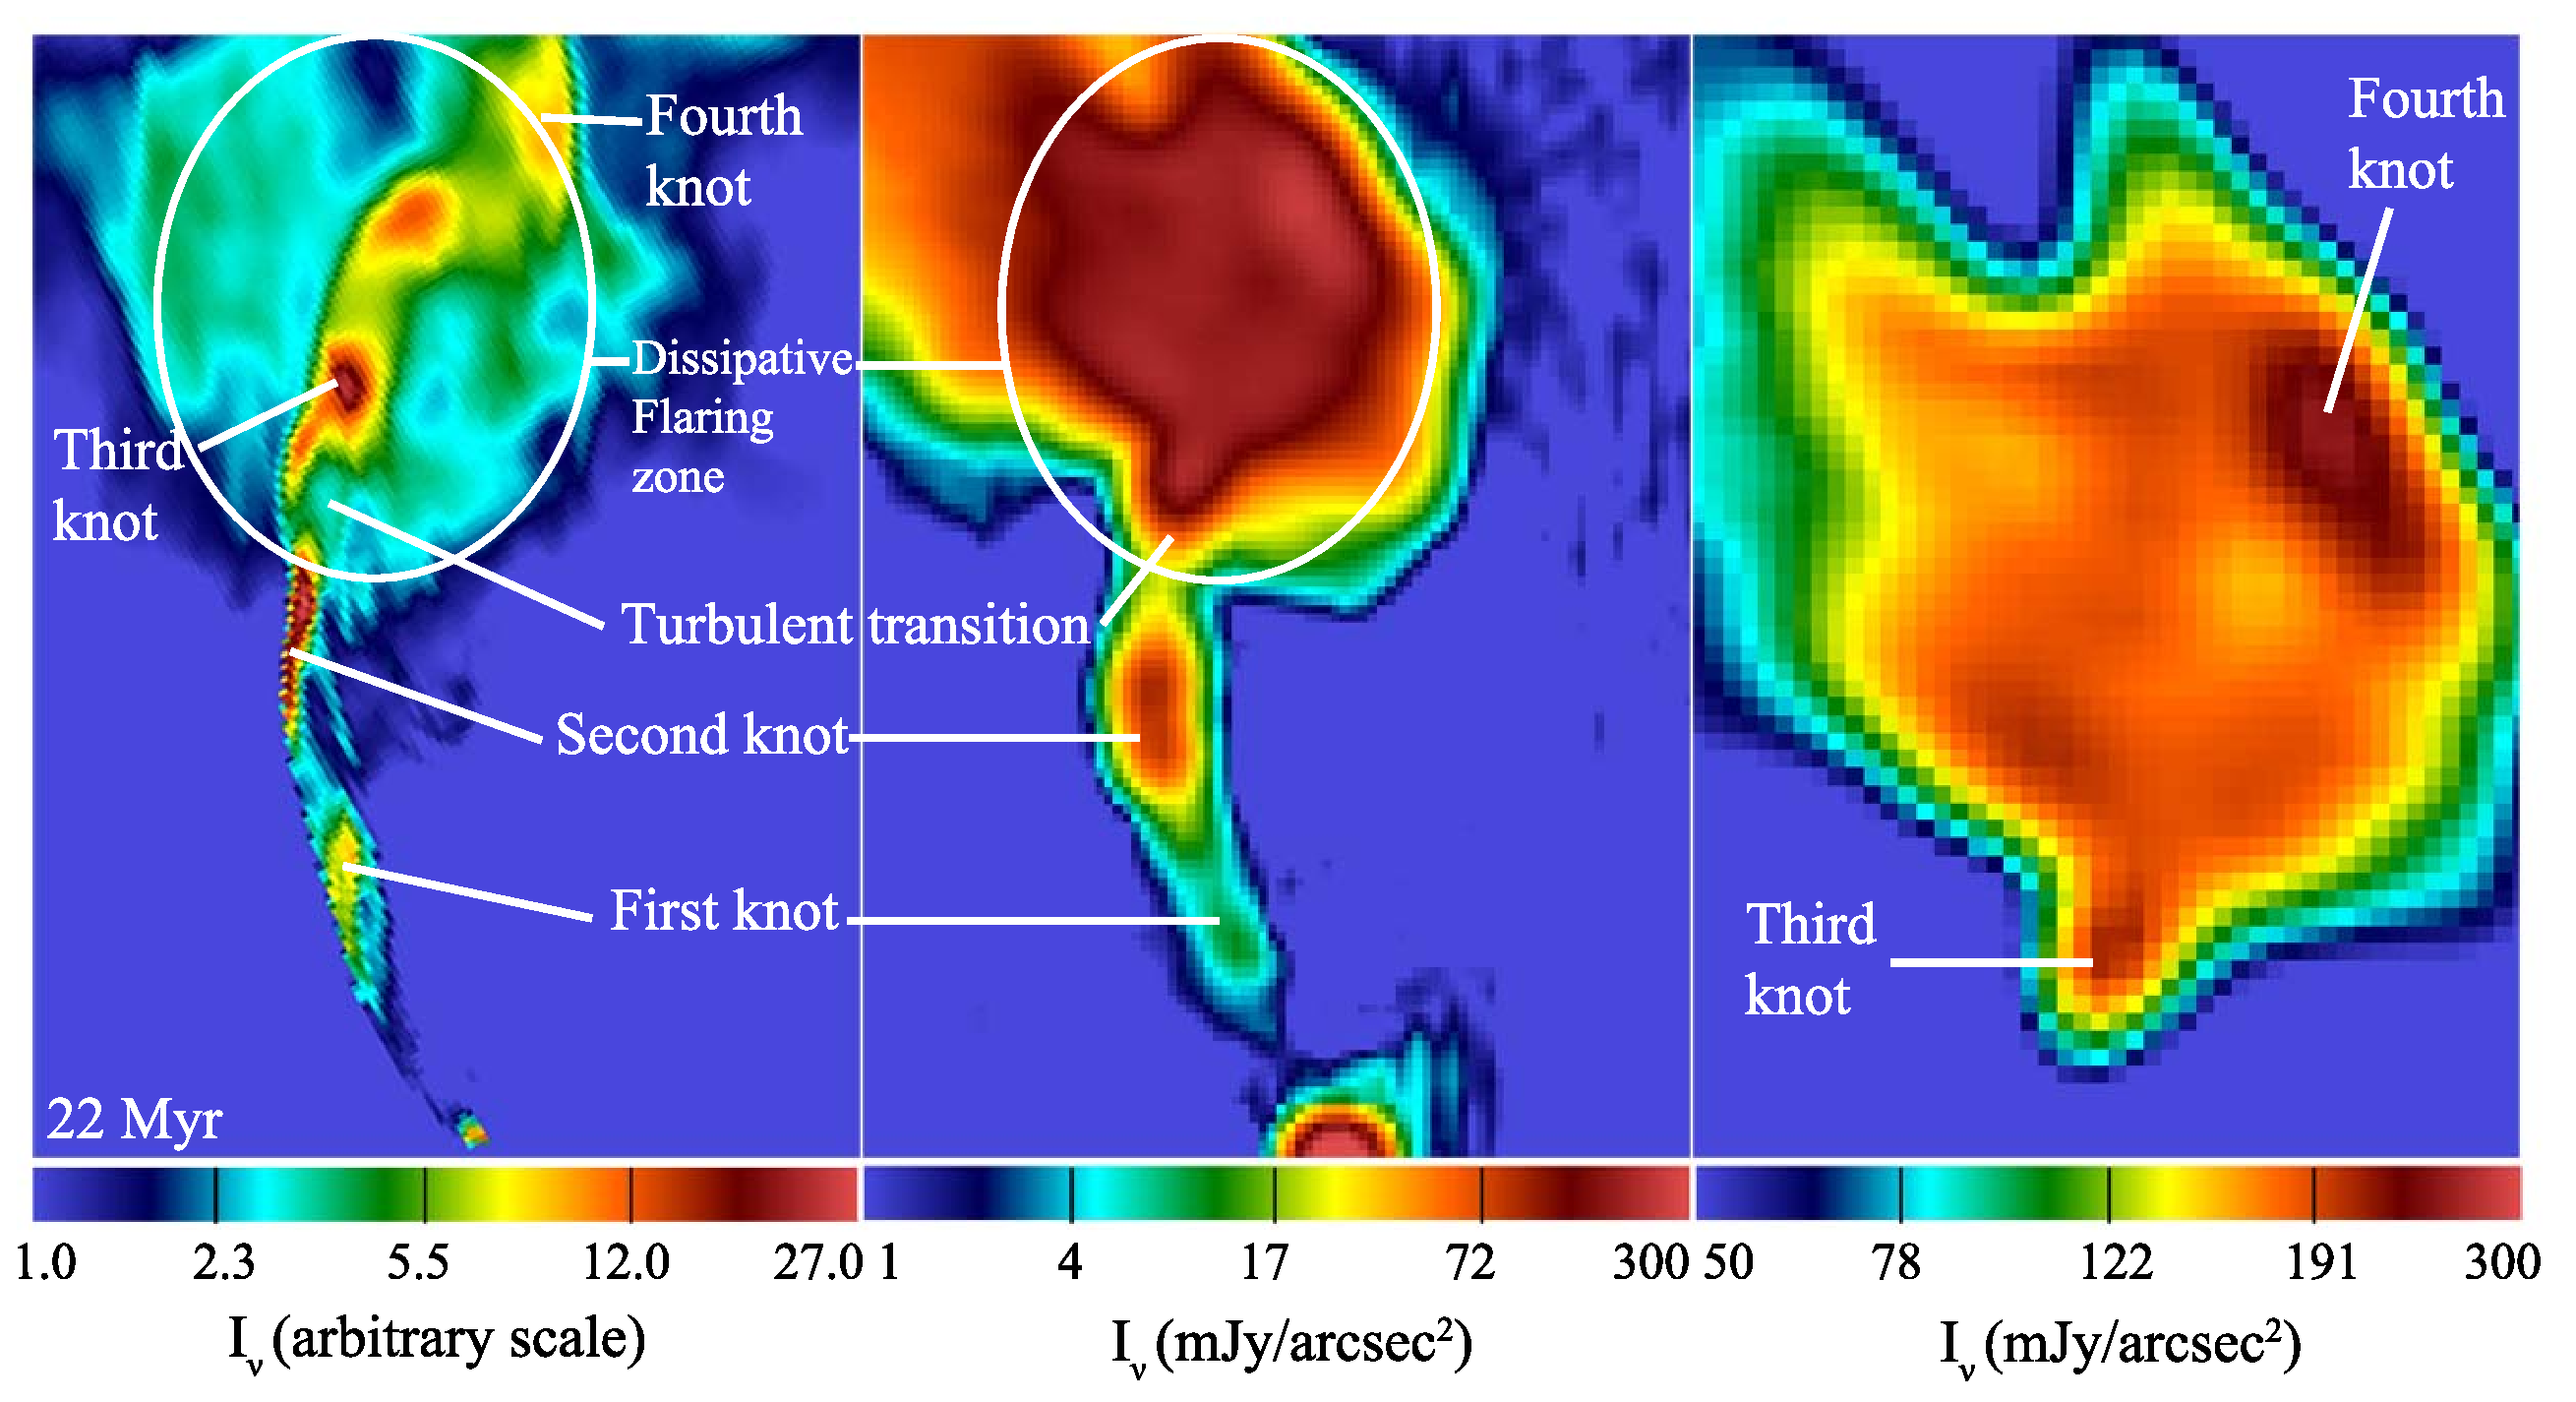
\includegraphics[width=\textwidth]{fig5.eps}
\caption{ A comparison between the source morphology of the best match model (run A, left panel) and the observational data by \citet{taylor90} (middle and right panel).}
\label{f:hyd}
\end{figure*}

\begin{figure*}
\centering
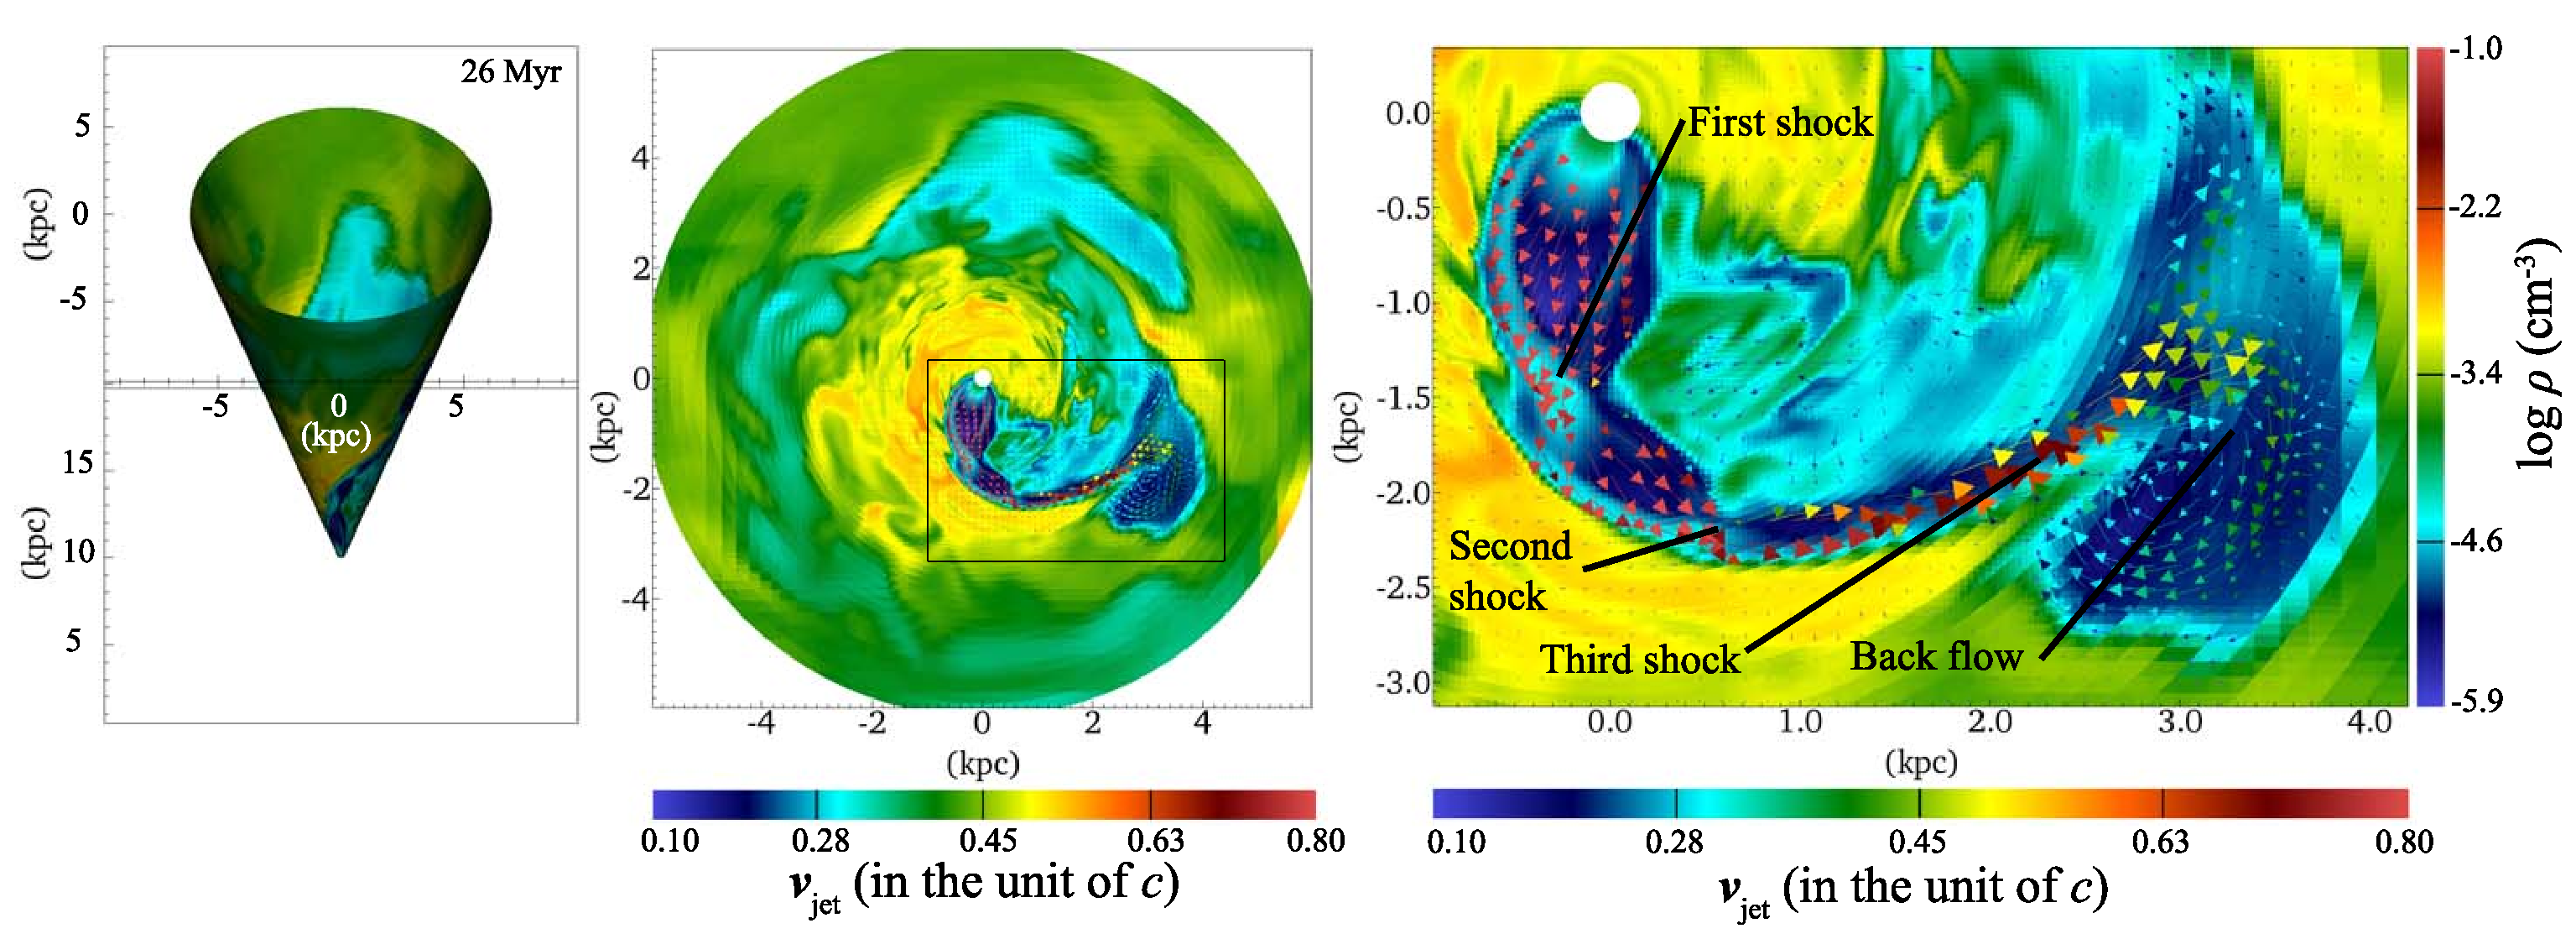
\includegraphics[width=\textwidth]{fig6.eps}
\caption{ Conic slice (cone angle 17$^{\circ}$ and cone axis aligned with the $z$-axis) of the logarithmic density image overlaid with the flow vector of the optimal model (model A) at a simulation time 26 Myr (left panel). The middle panel shows the projection of the cone onto the $x-y$ plane. The right panel is a zoom in image of the region marked by a rectangle in the middle panel.  }
\label{f:fdir}
\end{figure*}

Fig.~\ref{f:hyd} compares the optimal view of the simulated jet of model A (left panel, at a simulation time 22 Myr) and the Hydra A northern jet (middle and right panel). It is evident that the simulated jet successfully reproduces the following key features and processes occurring in the the source within the central 20~kpc. 

The moderately over-pressured precessing jet interacts with the ambient medium and produces four reconfinement shocks at approximately 4.0~kpc, 7~kpc, 10.0~kpc and 14.0~kpc from the core. Since the synchrotron emissivity is $j_{\nu} \propto p^{(3+\alpha)/2}$, downstream of the reconfinement shocks the pressure and therefore the surface brightness increase producing four bright knots. We see that the locations of the bright knots produced with this model agree well with the locations of bright knots in the Hydra A northern jet located at approximately 3.7~kpc, 7.0~kpc, 11.0~kpc and 16.0~kpc (deprojected) from the core and shown in the middle and right panel. In the simulated jet we see that a turbulent transition of the jet to a plume occurs approximately after the second bright knot, which is consistent with the observations.

% This figure also shows that in the optimal model, the turbulent jet starts to forms a dissipative flaring zone (marked by the ellipse in the left panel). This is the beginning of a large plume structure as observed in the Hydra A northern jet.

% Currently, we are investigating further development of the plume for an extended inner region (up to ~30kpc) of the northern jet with high resolution simulations. This will be presented in our next paper.

In the Hydra A northern jet, the flaring region within approximately 11 to 20~kpc from the core where the plume starts, is bright compared to the inner collimated jet. The corresponding region in the optimal model does not reach the same level of brightness. However, the flaring region is strongly turbulent (see \S~\ref{flaring}).
The amplification of the magnetic field resulting from this turbulence may be responsible for the increase in the source brightness. Since, my model is purely hydrodynamic, and the amplification of the magnetic field is not reflected in the synthetic surface brightness images. In order to produce more accurate synthetic brightness images magnetohydrodynamic (MHD) models are required. Therefore, further development of this model with the inclusion of magnetic field is of interest.

\subsection{Turbulent flaring zone}
\label{flaring}
Fig.~\ref{f:fdir} shows the logarithmic density of run A (at a simulation time 26 Myr) sliced by a cone with a cone angle of 17$^{\circ}$ (left panel) and cone axis aligned with the precession axis ($z$ axis). To obtain a clear view of the jet and the flow direction the cone is projected onto the $x-y$~plane (right panel of Fig.~\ref{f:fdir}) and overlaid with the flow vectors. A zoom in of the region marked by a rectangle in the middle panel is shown in the right panel. It is noted here that, although the precession angle in model A is 20$^{\circ}$, the jet is mostly visible along the conic slice with a cone angle 17$^{\circ}$. This is the result of the reflective boundary condition at the lower $z$ boundary. The reflection of the back flow on the side of the jet closest to the boundary pushes the jet towards the precession axis. Therefore, the jet is maximally visible along a conic slice with cone angle less than $20^{\circ}$. 

In Fig.~\ref{f:fdir} we see that after the turbulent transition of the jet some jet plasma hits the relatively dense cocoon plasma and produces a strong back flow (shown in the right panel). This turbulent back flow  establishes a flaring region. Such a flaring region is apparent at approximately 10 to 20~kpc from the core in the northern jet of Hydra A.
 Moreover, in the polarisation image of Hydra A \citep{taylor90} the polarisation significantly falls from 40$\%$ (in the collimated jet) to 10$\%$ in the flaring region. This reduction in polarisation suggests that the flaring region of the northern jet is turbulent and this is consistent with the simulations.  

%%%%%%%%%%%%%%%%%%%%%%%%%%%%%%
%
%			Forward shock
%
%%%%%%%%%%%%%%%%%%%%%%%%%%%%%%
\subsection{Forward shock} 
\begin{figure*}
\centering
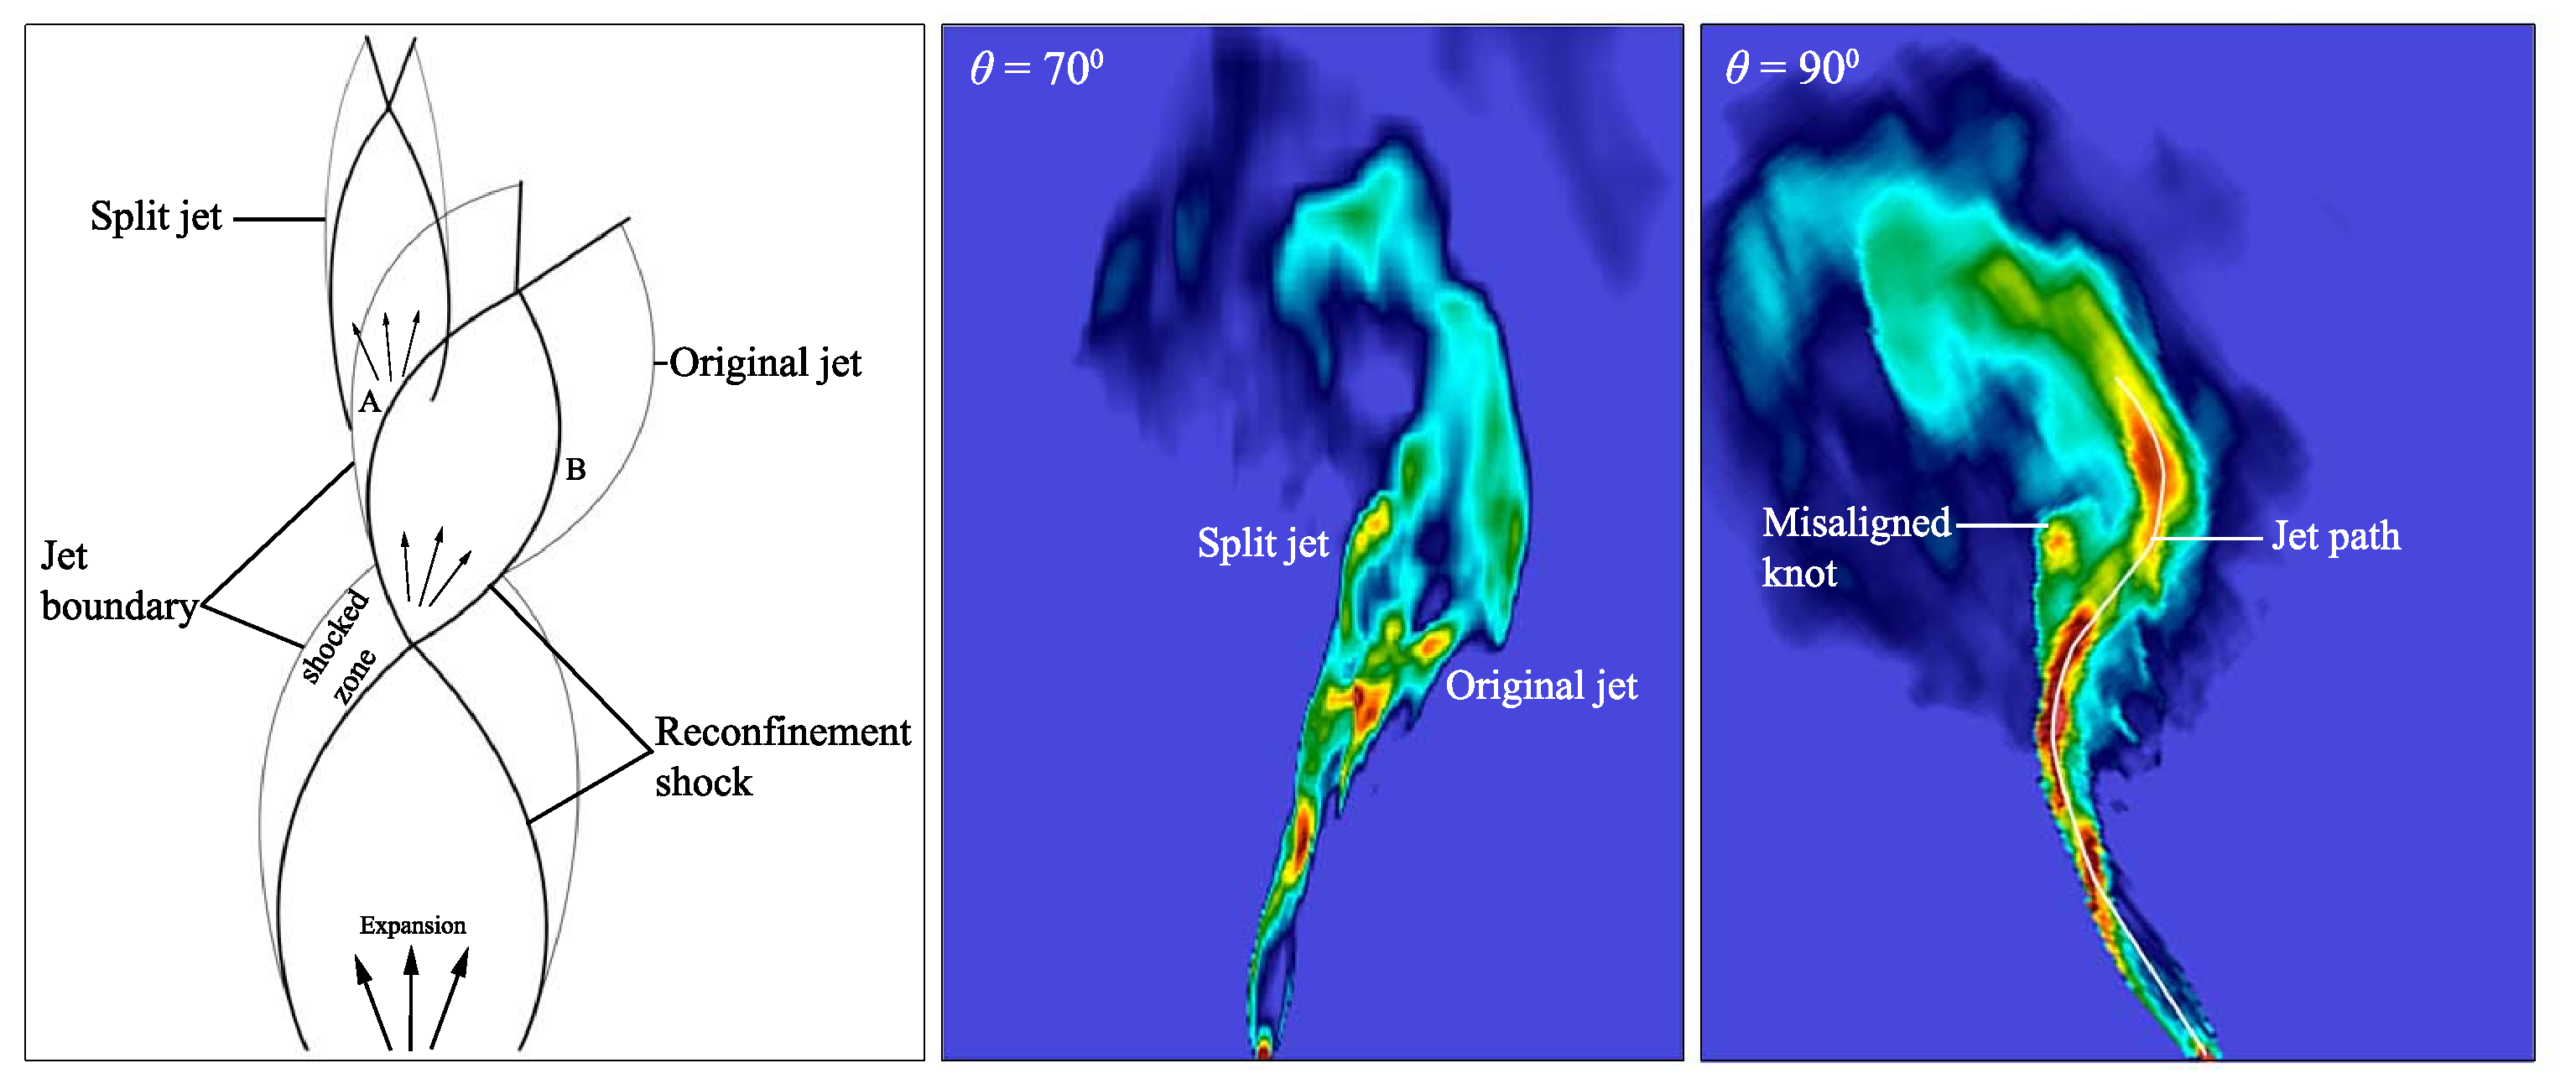
\includegraphics[width=\textwidth]{fig7.eps}
\caption{ Left: Midplane slice of the logarithmic density snapshot of model A. The forward bow shock is marked by an arrow in this panel. Right: Locations of the forward shock at five different time steps (points) . A least square linear fit (line) gives a shock advance speed $\approx$ 1630 km s$^{-1}$. }
\label{f:fsh}
\end{figure*}
%GVB
%In our best natch model the cocoon is separated from the ambient medium by an advancing forward shock. Here we estimate the Mach number of that forward shock. 

In the optimal model the radio jet-ICM interactions are bounded by an advancing forward shock. Here I estimate the Mach number of that forward shock. 

The forward bow shock is shown in the logarithmic density snapshot of model A (left panel of Fig.~\ref{f:fsh}). In the right panel of Fig.~\ref{f:fsh} the location of the forward shock along the $z$-axis at five different time steps is indicated. A least square fit to the shock positions gives a shock advance speed $\approx  1630$ km s$^{-1}$ of the forward shock. The sound speed at approximately 15~kpc from the core is $\approx 880$ km s$^{-1}$. Hence, the Mach number of the forward shock is $\approx 1.85$. 
There is a mild pressure jump $\approx 3.4$ at the forward shock. The low Mach number and mild pressure jump indicate that the heating of the atmosphere by the radio AGN in its earlier stage is gentle. This general feature of the heating of cooling flows was inferred by \citep{mcnamara12}. A straight jet would give a much higher advance speed and a larger pressure jump. The low Mach number and pressure jump derived here can be attributed to the jet precession depositing its momentum over a much wider area. 

%%%%%%%%%%%%%%%%%%%%%%%%%%%%%%
%
%			Mis-aligned knot
%
%%%%%%%%%%%%%%%%%%%%%%%%%%%%%%
\subsection{Misaligned bright knot}
\begin{figure*}
\centering
\includegraphics[width=\textwidth]{fig8.eps}
\caption{A misaligned knot produced by the jet splitting. In the left panel the jet splitting is shown in a synthetic surface brightenss image for a line of sight $\theta = 70^{\circ}$. In the right panel the synthetic surface brightness image is presented for a different line of sight $\theta = 90^{\circ}$, for which the jet path and the misaligned knot are clearly shown. }
\label{f:mknt}
\end{figure*}

In the turbulent flaring region of the Hydra A northern jet there is a  knot, which is not aligned with the main trajectory of the jet. This mis-aligned knot is approximately two kpc north of the third knot and is marked as 'misaligned knot' in Fig.~\ref{f:obs}. This knot is formed as a consequence of the transition to turbulence of the jet. The jet temporarily splits in two forming the misaligned knot and then returns to its final trajectory through the plume region (see Figure~\ref{f:mknt}). This happens only with the optimal model (A).

%Mis-aligned knots appear frequently in synthetic surface brightness images of our best matching model (run A). Models with higher precession periods (run C, D, E, F and G), and model with precession period 1~Myr but low precession angle (run B) do knot produce such mis-aligned knot. The mis-aligned knot usually appear in the flaring region of the jet and are short-lived  compared to the first couple of knots in the main jet at smaller radii. Close inspection of the flow evolution reveals that the jet occasionally splits in two - a main jet and a secondary jet, with the mis-aligned knot forming as a reconfinement shock in the secondary jet. Surveying the surface brightness image evolution of our simulations from a given line of sight, we find that jet splitting and the formation of mis-aligned knots occurs about 2 to 4 times per precession period. It is possible that the occurrence frequency is higher if we included counts along different lines of sights. The splitting of the jet always occurs near the region where the flow transitions to turbulence, and is often in the shape of a tuning fork. We can see that the mis-aligned knot is due to a reconfinement shock because the jet flow remains continuous along the split jet with knots forming at roughly the same distance from the fork. 
%
%The morphology of the split jet with reconfinement shocks forming in both the primary and secondary jet is sketched in panel 1 of Fig.~\ref{f:mknt}. The second and third panels of Fig.~\ref{f:mknt} show a snapshot example from model A (t = 26~Myr) at viewing angles of $\psi=70$ and $\psi=90$ respectively, in which the jet is split and has created two knots, one aligned with the precessional trajectory of the jet, and one clearly offset northward from the main jet. In Appendix~\ref{A:mknt}, we show further examples of the splitting of the jet and the formation of a mis-aligned knot, all at different snapshots from the model A.
%
%The reason for the splitting of the jet is difficult to pin down. Even the exact geometry of the splitting is difficult to reconstruct. We cannot easily determine the orientation of the splitting (i.e., the plane of the ``tuning fork''). Some snapshots of our simulations appear to indicate that the splitting occurs perpendicular to jet along the direction of precession (e.g. panels 2 and 3 Figure ??), In this case, the leading edge of the precessing jet, whose shocked region (region A in panel 1 of Fig.~\ref{f:mknt}) is highly overpressured, is perturbed, allowing the jet to channel, expand, and reconfine in a different direction to the original jet. Due to the incoming flow that compresses the shocked region at the leading edge of the precessing jet, that side is more overpressured than the shocked region of the receding edge (region B in panel 1 of Fig.~\ref{f:mknt}). The leading edge is also more exposed to perturbations as the precessing jet  moves into regions of turbulent backflow. A small blob of slightly denser gas back-flowing into the path of the jet would easily split the jet. This could naturally explain why we often see the split secondary jet emerge from the leading edge of the precessing primary jet. As the primary jet catches up with the split secondary jet, the latter is seen to evolve into the primary jet, while the other jet and its associated knot fades.
%
%The fact that the secondary jet evolves into the primary jet  may also suggests that jet  splitting and the formation of misaligned knots could, in fact, be a manifestation of jet jittering, helical bending of the jet caused by the Kelvin-Helmholtz shear instability \citep{begelman84, hardee13}. The bending would only be temporary because the jet flow keeps re-establishing itself as it precesses to propagate in a different direction. Alternatively, the appearance of knots may simply be related to transition to turbulence giving rise to random bifurcations to the flow direction of the marginally laminar jet. 

%%%%%%%%%%%%%%%%%%%%%%%%%%%%%%%%%%%%%%%%%%
%
%				Implication of precession
%
%%%%%%%%%%%%%%%%%%%%%%%%%%%%%%%%%%%%%%%%%%
\subsection{Implication of precession: Estimate of viscosity parameter of the AGN disk}
Knowledge of the precession period of the jet provides us with information that can be used to estimate the well known accretion disk viscosity parameter $\alpha$. A black hole (BH) whose spin is misaligned with the angular momentum of the accretion disk aligns the surrounding inner part of the disc to the BH spin axis via Lense-Thirring precession and internal viscosity up to a critical radius known as the Bardeen-Petterson radius, $r_\mathrm{BP}$ \citep{bardeen75}. Beyond $r_{\rm BP}$, the disk retains its original structure because of its dominant angular momentum. Viscous torques in the outer accretion disk force the spin axis of the black hole to precess until it is aligned with the angular momentum of the outer disk \citep{rees78, scheuer96, natarajan98, caproni07}. The alignment time-scale can be considered equivalent to the precession period of the jet. Using the alignment timescale, a jet precession period $\approx$ 10$^8$-10$^{10}$ yr has been estimated for the source, NGC 4258 \citep{caproni07}. 

%I use the theory of \citet{natarajan98} to estimate the accretion disk viscosity parameter $\alpha$. 
\citet{natarajan98} estimated the alignment time scale in terms of accretion parameters, including the disk viscosity parameter, $\alpha$. Using their theory, I use the precession period of the optimal model of Hydra A to estimate $\alpha$. 
Let $t_{\rm align}$ be the alignment time-scale, $a$ the spin parameter of the black hole, $\alpha$ the viscosity parameter of the accretion disk, $L$ the total power provided by the black hole,
%($L_{\rm bol}$ + $L_{\rm jet}$), where $L_{\rm bol}$ is the bolometric luminosity of the source, and $L_{\rm jet}$ is the jet kinetic power 
$L_{\rm E}$ the Eddington luminosity, $M_{\rm BH}$ the mass of the black hole, $M_{\odot}$ the solar mass, and $\epsilon$ the accretion efficiency of the black hole. Then, from the equation for the alignment time of the black hole (\citealt[][equation 2.16]{natarajan98}) I obtain:
\begin{align}
\alpha & = 0.04 \left(\frac{a}{0.8}\right)^{-11/26} \left(\frac{L}{0.02 L_{\rm E}}\right)^{7/13} \\ \nonumber 
           & \times \left(\frac{M}{ 10^9 M_{\odot}}\right)^{1/26}  \left(\frac{\epsilon}{0.1}\right)^{-7/13} \left(\frac{P}{\rm Myr}\right)^{8/13}\:.
\end{align}
where $P(=t_\mathrm{align}$) is the precession period of the jet.

The mass of the supermassive black hole in Hydra A is approximately $10^9$ M$_{\odot}$ \citep{fujita13}.
The total jet power provided by the black hole is $L=2L_{\rm jet}\approx 2 \times 10^{45}$ erg s$^{-1}\approx 0.02L_{\rm E}$ and I equate this to the total disk luminosity resulting from accretion. Using $\epsilon = 0.1$, $P=1$~Myr, and a range of $a$ (= 0.1 to 1) I obtain $0.03\le \alpha \le 0.15$. The upper end of the range of $\alpha \approx 0.15$ (for $a \approx 0.1$) is consistent with the range of values typically inferred from observations of dwarf novae $0.1\le \alpha \le 0.4$ \citep{king07}. However, in general, there is a discrepancy between values of $\alpha$ derived from observations and those derived from numerical magneto-hydrodynamic (MHD) simulations; the latter are generally an order of magnitude lower than the former. For instance, the quasi-steady disk MHD models by \citet{parkin13b} imply $\alpha \approx 0.04$. Such a low value is consistent with the lower bound of the estimate of $\alpha$ (for $a\approx 0.9$). The lowest value $\alpha = 0.03$ in the range is consistent with the estimates by \citet{starling04} from observations of AGN disks.


%%%%%%%%%%%%%%%%%%%%%%%%%%%%%%%%%%%%%%%%%
%
%				Appendices
%
%%%%%%%%%%%%%%%%%%%%%%%%%%%%%%%%%%%%%%%%%
\newpage
%\centering{Appendices}
\begin{appendices}
\section{Rotation of the data cube for a desired line of sight}\label{A:trans}
\begin{figure*}
\centering
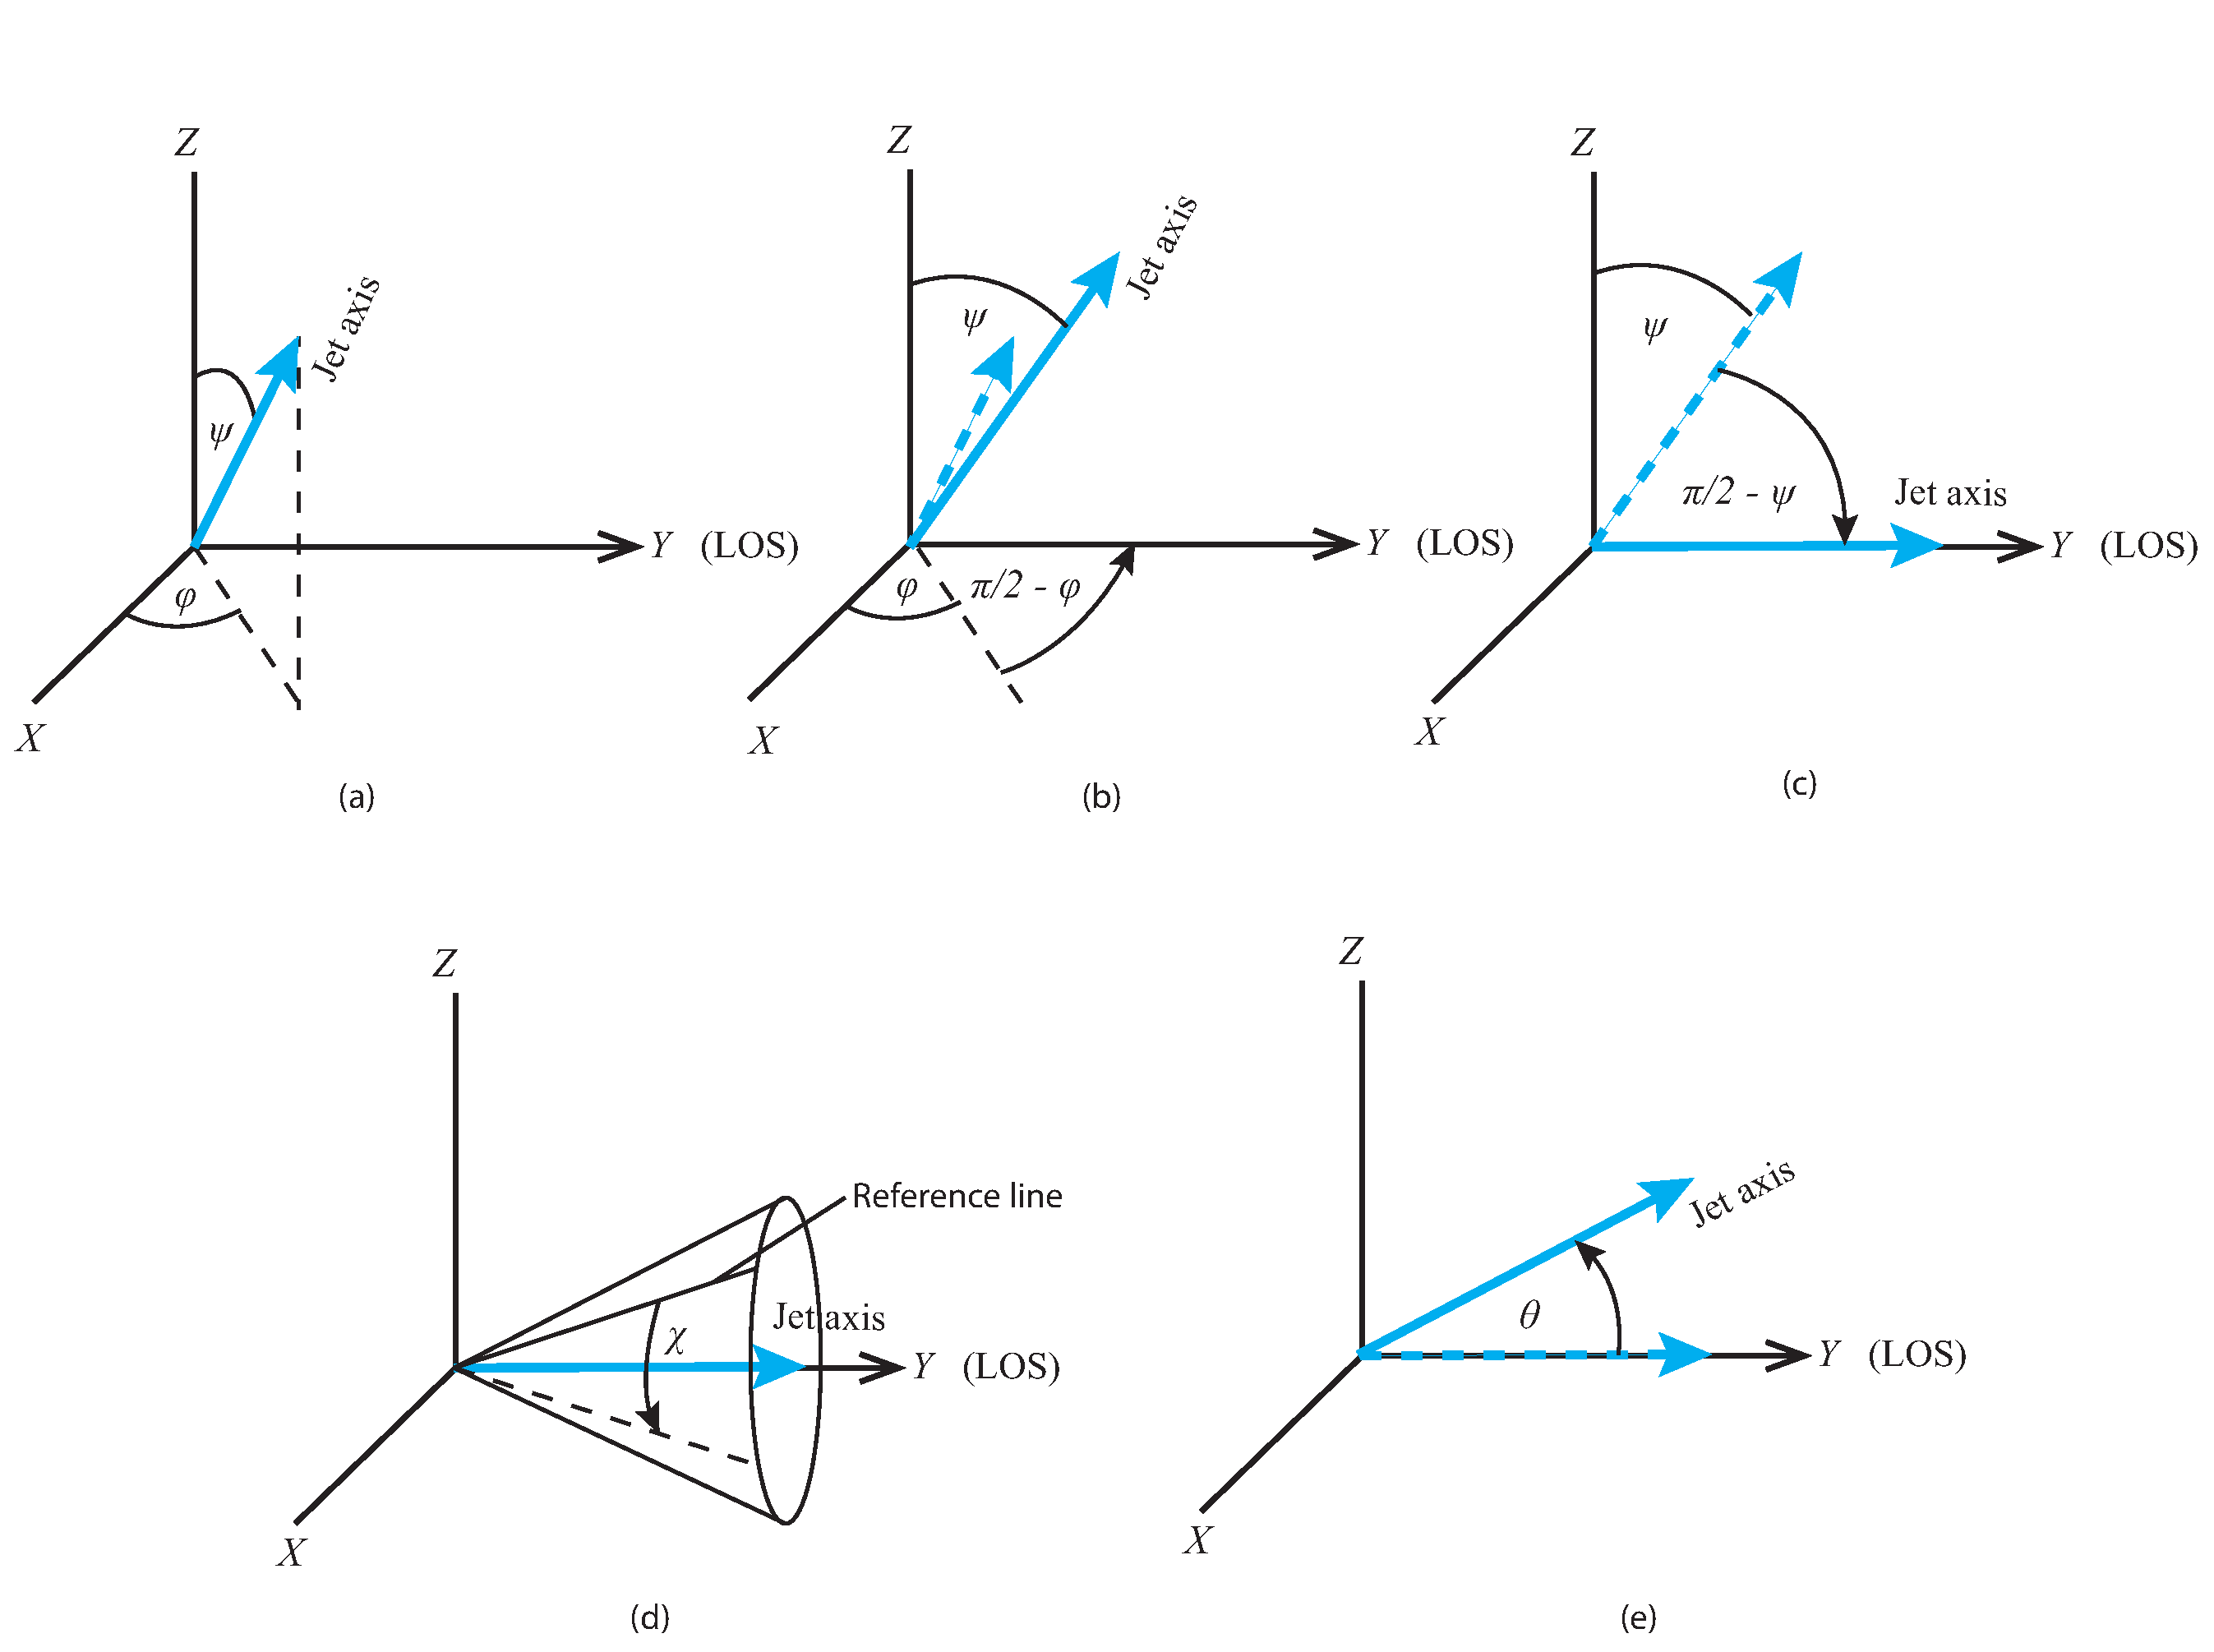
\includegraphics[width=\textwidth]{fig9.eps}
\caption{Transformations associated with the rotations of points of the simulation data cube with respect to the synthetic image cube. Panel (a): At a given instant, both the data cube and the image cube have the same orientation and they can be represented by the same coordinates $XYZ$. Panel (b): Transformation associated with the angle $\phi$, to bring the jet axis on the $YZ$ plane. Panel (c): Transformation associated with the angle $\psi$, to align the jet axis with the line of sight $Y$ axis. Panel (d): Transformation associated with the angle $\chi$, to obtain a desired viewing direction. Panel (e): Transformation associated with the angle $\theta$, to obtain a desired line of sight. In panels (b), (c) and (e) the jet axes before transformations are shown in dashed blue arrows and after transformations with solid blue arrows. In panel (d), the jet does not change its location. It only rotates about its axis. }
%\caption{Transformations of the coordinates associated with the data cube ($xyz$) with respect to coordinates associated with the image cube ($XYZ$) to obtain a line of sight $\theta$ and a viewing direction $\chi$. The line of sight is along the $Y$ axis. See text in Appendix~\ref{A:trans} for details.  }
\label{f:rot}
\end{figure*}
%Let $xyz$ be the coordinates (shown in panel (a) of Fig.~\ref{f:rot}) associated with the simulation data cube. At a given time the jet (shown in a blue thick line in panel (a)) makes angles $\psi$ and $\phi$ with the $z$ and $x$ axes. Let $XYZ$ be the coordinates (shown in panel (a) of Fig.~\ref{f:rot}) associated with the synthetic image cube. 
%To obtain a desired line of sight and viewing direction we perform the following rotations of the simulation data cube with respect to the synthetic image cube. These rotations are depicted in Fig.~\ref{f:rot}. In each panels of this figure the coordinates associated with the image cubes are shown in bold solid lines, the coordinates associated with the simulation data cubes are in solid (before transformations) and dashed (after transformations) lines, the jets before transformations are in light blue thick lines and the jet after transformations are in dark blue thick lines. 
%Transformations of the coordinates associated with the data cube ($xyz$) with respect to coordinates associated with the image cube ($XYZ$) to obtain a line of sight $\theta$ and a viewing direction $\chi$. The line of sight is along the $Y$ axis. See text in Appendix~\ref{A:trans} for details. 

Let $XYZ$ be the coordinates (shown in panel (a) of Fig.~\ref{f:rot}) associated with the synthetic image cube, onto which the ray trace integration is performed. Let $Y$ is the direction of the line of sight. At a given instance the synthetic image cube and the simulation data cube have the same orientation. Hence, at that given instance the direction and location of the jet is defined by the precession angle $\psi$, angle between the jet axis and the precession axis $Z$, and an angle $\phi$ with respect to a fixed axis (say $X$-axis, see panel (a) of Fig.~\ref{f:rot}). Let $\chi$ be the angle defining viewing direction, an angle about the line of sight. To make the angle $
\chi$ understandable, I introduce a viewing cone and a reference line in panel (d) of Fig.~\ref{f:rot}. $\chi$ is then an angle with respect to the reference line. Let $\theta$ be the angle between the jet axis and the line of sight $Y$-axis (see panel (e) of Fig.~\ref{f:rot}).

In order to obtain a desired line of sight $\theta$ and viewing direction $\chi$ I perform the rotations of the data cube with respect to the image cube. In other words, I perform rotations of points (known as \emph{point transformation\footnote{For an anti-clockwise rotation of points by an angle $\theta$ about the origin of a two dimensional coordinate system $XY$, the rotation matrix is given by \begin{eqnarray}
R = \begin{pmatrix}
 \cos\theta & -\sin\theta \\
\sin\theta & \cos\theta \nonumber \\
\end{pmatrix}.
\end{eqnarray}}})
%For a counter-clockwise rotation of a two dimensional coordinate system $XY$ by an angle $\theta$ while the points are fixed, the rotation matrix is given by
%\begin{eqnarray}
%R = \begin{pmatrix}
% \cos\theta & \sin\theta \\
%-\sin\theta & \cos\theta. \nonumber \\
%\end{pmatrix}
%\end{eqnarray}}} ) 
of the data cube with respect to the fixed image cube. 

Since the visualisation software VISIT restricts the choice of the line of sight along any one axis of the image cube (in my case I choose $Y$-axis), we require four rotations; two rotations associated with $\psi$ and $\phi$ to align the jet axis with the line of sight and two rotations associated with $\chi$ and $\theta$ to obtain the desired viewing direction and line of sight. These rotations are depicted in Fig.~\ref{f:rot}. In this figure angles are depicted by arcs and rotations are depicted by arcs with arrowheads. 

%In a point transformation (or, rotation), actual points are rotated with respect to a fixed coordinate system (unlike a nsformation where points are fixed and the coordinates are transformed).  

%Since the choice of the line of sight with the visualisation software VISIT is restricted among any of the axes of the image cube, I choose $Y$ axis as the direction of the line of sight.
%The direction and location of the jet at a given moment is defined by the precession angle $\psi$ and an angle $\phi$ with respect to a fixed axis (say $X$-axis). 
%
%At a given instance the direction and location of the jet (shown by jet axis in each panel) is defined by the precession angle $\psi$ and an angle $\phi$ with respect to an arbitrary axis (say wrt X). 
%
%The choice of the line of sight with the visualisation software VISIT is restricted among any of the axes of the image cube. I choose $Y$ axis as the direction of the line of sight.
%
%Prior to perform any transformation  the synthetic image cube and the simulation data cube have the same orientation. 
%\begin{enumerate}
%\item At a given time the location of the jet is defined by its precession angle $\psi$ and the azimuth angle $\phi$ with respect to $X$ (shown in panel (a)).
%\item  
%\end{enumerate}

% 

%The line of  At a given instance 

%At a given instance the jet (shown in thick blue lines of each panel of Fig.~\ref{f:rot}) makes angles $\psi$ and $\phi$ with the $z$ and $x$ axes. 
%
%At a given time the data cube and the image cube are the same.  In order to obtain a desired viewing direction and line of sight I perform the following rotations of the simulation data cube with respect to the synthetic image cube. 
%
%  At a given time the jet (shown in a blue thick line in panel (a)) makes angles $\psi$ and $\phi$ with the $z$ and $x$ axes. In order to obtain a desired viewing direction and line of sight we require to perform transportation of the data cube with respect to the synthetic image cube.  
%  
%  Let $XYZ$ be the coordinates (shown in panel (a) of Fig.~\ref{f:rot}) associated with the synthetic image cube. 
%To obtain a desired line of sight and viewing direction we perform the following rotations of the simulation data cube with respect to the synthetic image cube. These rotations are depicted in Fig.~\ref{f:rot}. In each panels of this figure the coordinates associated with the image cubes are shown in bold solid lines, the coordinates associated with the simulation data cubes are in solid (before transformations) and dashed (after transformations) lines, the jets before transformations are in light blue thick lines and the jet after transformations are in dark blue thick lines. 
\begin{enumerate}
\item First I rotate the simulation data cube (anticlockwise) with respect to the $Z$-axis by an angle $\pi/2 - \phi$ (shown in panel (b)). %The coordinates associated with the simulation data cube $xyz$ are transformed to $x'y'z'$. 
This rotation brings the jet axis on the $YZ$ plane. The rotation matrix for this rotation $R^{(AC)}_{Z(\pi/2 - \phi)}$ (here the superscript AC denotes the anticlockwise rotation) is given by 
\begin{eqnarray}
R^{(AC)}_{Z(\pi/2 - \phi)}  &=& \begin{pmatrix}
 \cos(\pi/2 - \phi) & -\sin(\pi/2 - \phi) & 0 \\
\sin(\pi/2 - \phi) & \cos(\pi/2 - \phi) & 0 \\
0 & 0 & 1
\end{pmatrix} \nonumber \\
&=& \begin{pmatrix}
 \sin\phi & -\cos\phi & 0 \\
\cos\phi & \sin\phi & 0 \\
0 & 0 & 1
\end{pmatrix} 
\end{eqnarray}
\item I rotate the simulation data cube second time (clockwise) with respect to the $X$-axis by an angle $\pi/2 - \theta$ (shown in panel (c)). 
%The coordinates associated with the simulation data cube $x'y'z'$ are transformed to $x''y''z''$. 
This rotation makes the jet axis aligned with the line of sight $Y$-axis. The rotation matrix for this rotation $R^{(C)}_{X(\pi/2 - \psi)}$ (the superscript C denotes the clockwise rotation) is given by 
\begin{eqnarray}
R^{(C)}_{X(\pi/2 - \psi)} &=& \begin{pmatrix}
 1 & 0 & 0 \\
0 & \cos(\pi/2 - \psi) & \sin(\pi/2 - \psi) \\
0 & -\sin(\pi/2 - \psi) & \cos(\pi/2 - \psi)
\end{pmatrix} \nonumber \\
& = &\begin{pmatrix}
1 & 0 & 0 \\
0 & \sin\psi & \cos\psi \\
0 & -\cos\psi & \sin\psi
\end{pmatrix}  
\end{eqnarray}
\item Now to obtain a viewing direction I rotate the simulation data cube with respect to the $Y$-axis by an angle $\chi$ (shown in panel (d)). 
%The coordinates associated with the simulation data cube $x''y''z''$ are transformed to $x'''y'''z'''$. 
The rotation matrix for this rotation $R^{(AC)}_{Y(\chi)} $ is given by
\begin{equation}
R^{(AC)}_{Y(\chi)} = \begin{pmatrix}
 \cos\chi & 0 & \sin\chi \\
0 & 1  & 0 \\
-\sin\chi & 0 & \cos\chi
\end{pmatrix}  
\end{equation}
\item Finally, I rotate the simulation data cube with respect to the $X$-axis by and angle $\theta$ (shown in panel (e)). This rotation relocates the jet axis at an angle $\theta$ with respect to the $Y$-axis (line of sight). 
%The coordinates associated with the simulation data cube $x'''y'''z'''$ are transformed to $x''''y''''z''''$. 
The rotation matrix associated with this rotation $R'^{(AC)}_{X(\theta)}$ is given by
 \begin{equation}
  R'^{(AC)}_{X(\theta)} = \begin{pmatrix}
 1 & 0 & 0 \\
0 & \cos\theta & -\sin\theta \\
0 & \sin\theta & \cos\theta 
\end{pmatrix}  
\end{equation}
\end{enumerate} 

The velocity of the fluid in the synthetic image cube $\textbf{v}'$ after the transformations described above is estimated from the velocity in the simulation data cube by using the rotation matrix $R = R'^{(AC)}_{X(\theta)} R^{(AC)}_{Y(\chi)} R^{(C)}_{X(\pi/2 - \psi)} R^{(AC)}_{Z(\pi/2 - \phi)}$
\begin{equation}
\textbf{v}' = R \textbf{v}
\end{equation}

Let $s_1 = \sin \psi$, $s_2 = \sin \phi$, $s_3 = \sin \chi$, $s_4 = \sin \theta$, $c_1 = \cos \psi$,  $c_2 = \cos \phi$, $c_3 = \cos \chi$, and $c_4 = \cos\theta$. Then the rotation matrix $R$ is given by:
 \begin{eqnarray}
  R &=&  R'^{(AC)}_{X(\theta)} R^{(AC)}_{Y(\chi)} R^{(C)}_{X(\pi/2 - \psi)} R^{(AC)}_{Z(\pi/2 - \phi)} \nonumber \\
  &=&  \begin{pmatrix}
  c_3 s_2 - s_3 c_1 c_2  & -c_3 c_2 -s_3 c_1 s_2 & s_3 s_1 \\[6pt]
  c_4 s_1 c_2 + s_4 s_3 s_2  &  c_4 s_1 s_2 + s_4 s_3 c_2 & c_4 c_1 - s_4 c_3 s_1  \\
\phantom{{}+{}}+ s_4 c_3 c_1 c_2 & \phantom{{}+{}}- s_4 c_3 c_1 s_2  & & \\[6pt]
   s_4 s_1 c_2 - c_4 s_3 s_2 & s_4 s_1 s_2 + c_4 s_3 c_2  &  s_4 c_1 + c_4 c_3 s_1 \\
\phantom{{}+{}} - c_4 c_3 c_1c_2   &\phantom{{}+{}}-c_4 c_3 c_1 s_2  & & \\
\end{pmatrix} \nonumber 
\end{eqnarray}

% \begin{eqnarray}
%  R &=&  R'^{(AC)}_{X(\theta)} R^{(AC)}_{Y(\chi)} R^{(C)}_{X(\pi/2 - \psi)} R^{(AC)}_{Z(\pi/2 - \phi)} \nonumber \\
%  &=&  \begin{pmatrix}
%  c\chi s\phi - s\chi c\psi c\phi  & -c\chi c\phi -s\chi c\psi s\phi & s\chi s\psi \\[6pt]
%  c\theta s\psi c\phi + s\theta s\chi s\phi  &  c\theta s\psi s\phi + s\theta s\chi c\phi & c\theta c\psi - s\theta c\chi s\psi  \\
%\phantom{{}+{}+{}}+ s\theta c\chi c\psi c\phi & \phantom{{}+{}+{}}- s\theta c\chi c\psi s\phi  & & \\[6pt]
%   s\theta s\psi c\phi - c\theta s\chi s\phi & s\theta s\psi s\phi + c\theta s\chi c\phi  &  s\theta c\psi + c\theta c\chi s\psi \\
%\phantom{{}+{}+{}} - c\theta c\chi c\psi c\phi   &\phantom{{}+{}+{}}-c\theta c\chi c\psi s\phi  & & \\
%\end{pmatrix} \nonumber 
%\end{eqnarray}

%where $s$ and $c$ stands for $\sin$ and $\cos$ respectively. 

% \cos\chi \sin\phi - \sin\chi \cos\psi \cos\phi  & -\cos\chi \cos\phi -\sin\chi \cos\psi \sin\phi & \sin\chi \sin\psi \\

\newpage
\section{Synthetic surface brightness of the source at different $\theta$ and $\chi$}\label{A:morph}
\begin{figure*}
\centering
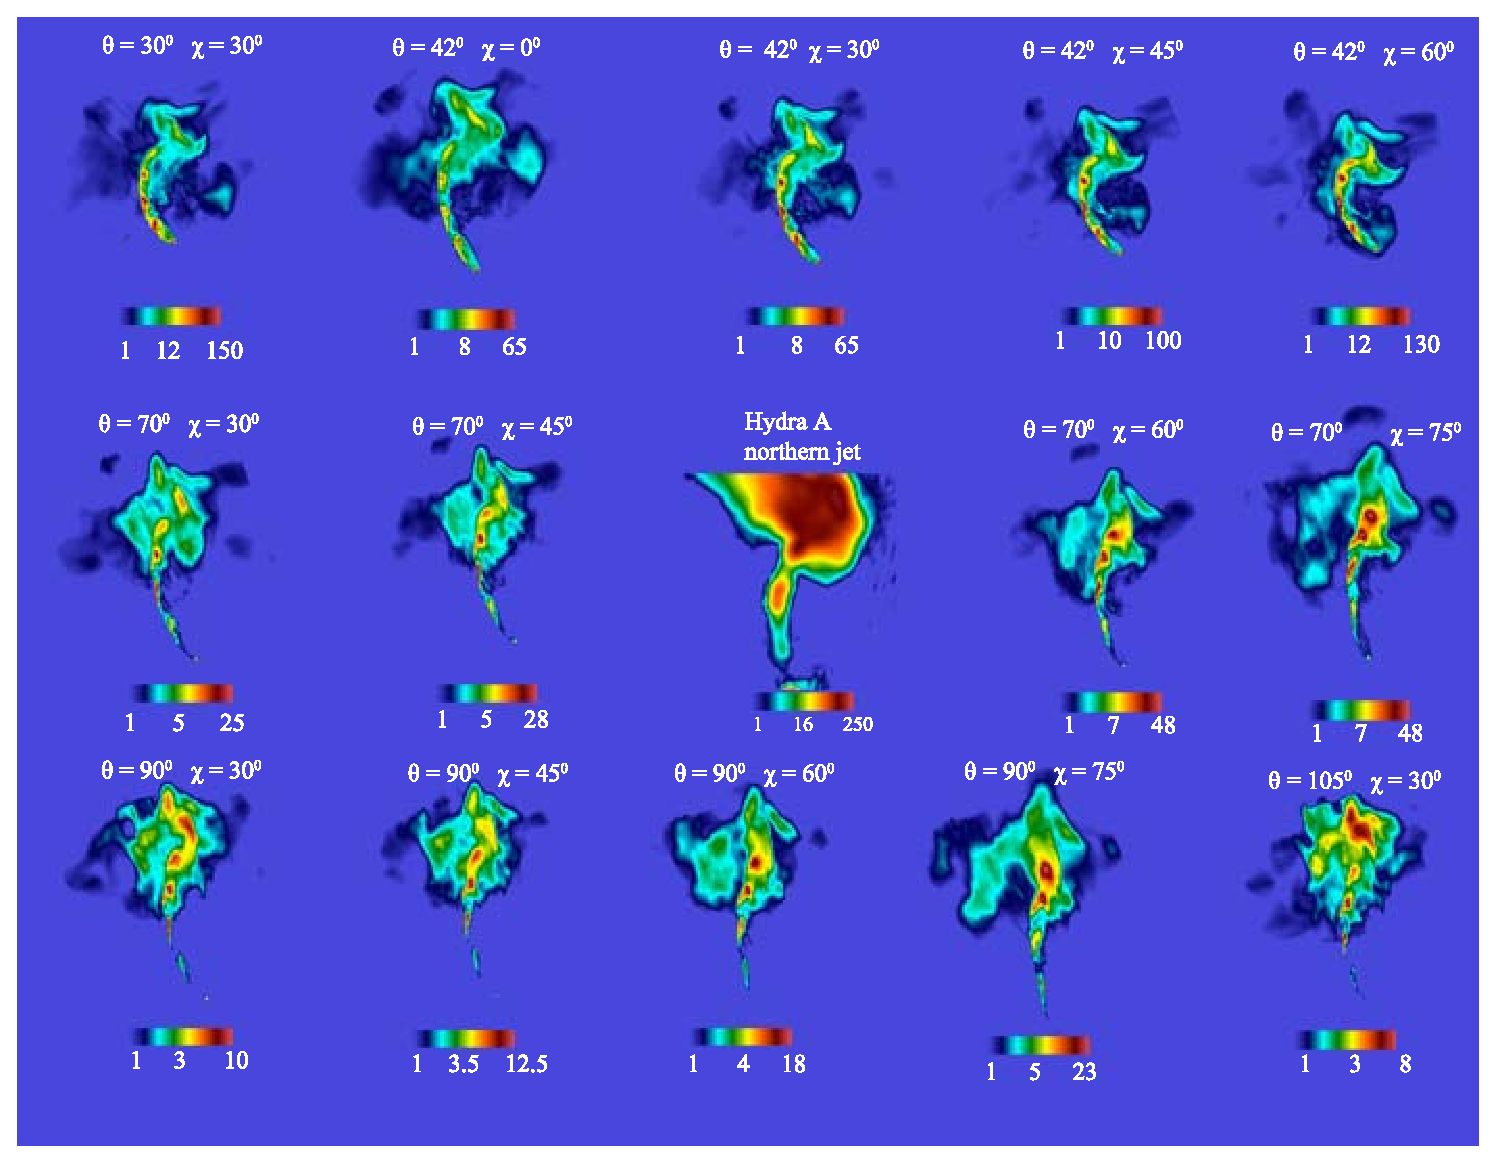
\includegraphics[width=\linewidth]{fig10.eps}
\caption{ Synthetic surface brightness images of the best match model for different line of sights $\theta$ and viewing directions $\chi$. For comparison the observed radio image of the inner 20~kpc of the Hydra A northern jet is shown at the third column of second row. }
\label{f:morph}
\end{figure*}






\end{appendices}